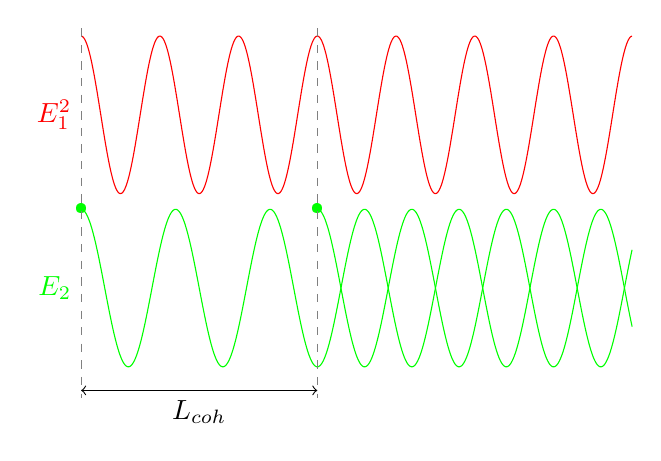
\begin{tikzpicture}[
indic/.style = {gray, dashed}
]
\def\xe{7}

%\fill[black!20] (0,1.1) rectangle (\xe,-3.3);
\draw[color=red] node[left] {$E_1^2$}  plot[samples=1000, domain=0:\xe] (\x,{cos(360* \x)});
%\draw[color=green] (0,-2.2) node[left,text width=1.7 cm] {$E_2$}  plot[samples=1000, domain=0:6] (\x,{cos(300* \x)-2.2});
\draw[color=green] (0,-2.2) node[left] {$E_2$} node at (0,-1.2) {\textbullet} plot[samples=1000, domain=0:\xe] (\x,{cos(300* \x)-2.2});
\draw[color=green] node at (3,-1.2) {\textbullet} plot[samples=1000, domain=3:\xe] (\x,{cos(300* \x + 180)-2.2});
\draw[indic] (3,1.1) -- (3,-3.6);% node {$z=L_\mathsc{coh}$};
\draw[indic] (0,1.1) -- (0,-3.6);% node {$z=0$};
\draw [<->] (0,-3.5) -- +(3,0) node[midway,below] {$L_\mathsc{coh}$};
%\draw (current bounding box.north east) rectangle (current bounding box.south west);
\end{tikzpicture}